% tikz: satisfiability implication digraphs
\documentclass[12pt]{article}
\usepackage{calc}
\usepackage{tikz}
\usetikzlibrary{arrows,decorations.markings}
\tikzstyle{vertex}=[circle, draw, inner sep=0pt, minimum size=18pt]
\newcommand{\vertex}{\node[vertex]}
\newcounter{Angle}

\pagestyle{empty}
\begin{document}
{%\large\bf
\[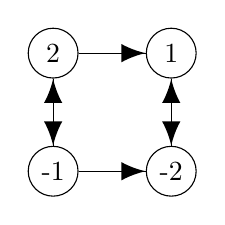
\begin{tikzpicture}[x=1.5cm, y=1.5cm
    ,every edge/.style={
        draw,
        postaction={decorate,
                    decoration={markings,mark=at position 1 with
		    {\arrow[line width=2pt,black]{latex}}} } }
]
\vertex (a) at (0,0) {-1};
\vertex (b) at (0,1) {2};
\vertex (c) at (1,0) {-2};
\vertex (d) at (1,1) {1};
\path
(a) edge (b) edge (c)
(b) edge (a) edge (d)
(c) edge (d)
(d) edge (c)
;
\end{tikzpicture}\]
\[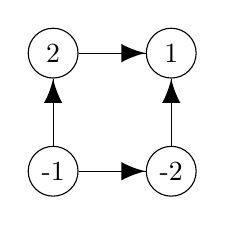
\begin{tikzpicture}[x=1.5cm, y=1.5cm
    ,every edge/.style={
        draw,
        postaction={decorate,
                    decoration={markings,mark=at position 1 with
		    {\arrow[line width=2pt,black]{latex}}} } }
]
\vertex (a) at (0,0) {-1};
\vertex (b) at (0,1) {2};
\vertex (c) at (1,0) {-2};
\vertex (d) at (1,1) {1};
\path
(a) edge (b) edge (c)
(b) edge (d)
(c) edge (d)
;
\end{tikzpicture}\]
\end{document}
